\chapter{System characterization and results}

In this chapter, efforts to characterize the performance and capabilities of the FO-DOCM device will be detailed. Results obtained with the FO-DOCM device on actual cochlear tissues will be shown. The shortcomings and successes of the apparatus will be detailed, and conclusions will be drawn.

\section{Resolution verification}

\subsection{Verification of axial resolution}

In Section \ref{sec:axial_res}, predicitions were made about the axial resolution achievable by the FO-DOCM system. Here, these predictions are validated and limitations are explained.

% \subsection{Results without AOMs}

% To prevent possibly confounding factors, the system was first tested with the AOMs in place. In this case, the $z$-axis stage was moved in increments of 100 nanometers and the DC voltage from the photodetector was acquired and stored for reach position. This ensures that the distance measured by the $z$-stage is accurate, but requires a smaller overall system gain so as not to saturate the photo-detector. The ``sample'' has been replaced by a mirror for maximum possible SNR.

% \begin{figure}[h!]
% \centering
% \includegraphics[width=0.75\textwidth]{Images/missing.png}
% \caption[The point spread function without acousto optic modulators.]{The point spread function without acousto optic modulators. The measured PSF is shown in black, the best fit Gaussian in green, and the predicted PSF in blue.}
% \end{figure}

% With this method, a full width half maximum PSF width of ?8.4? microns was measured. The calculated PSF is noisy as a result of the envelope detection method -- since the carrier frequency without AOMs is so much closer to the bandwidth of the PSF, the analytic signal extraction is much less exact. Furthermore, the variability in the stage position (on the order of 100nm) results in phase noise in the carrier wave, creating a much noisier signal. 

% \subsection{Results with AOMs}

To verify the axial resolution, the sample was replaced by an aluminum mirror. The $z$-axis stage was moved in increments of 100nm in a 60 micron range around the interference maximum. A small 0.1 second sample of the 500 KHz carrier wave was recorded for each position, from which the envelope could be extracted at each point.

The measured PSF, and a comparison to the PSF predicted in Section~\ref{sec:axial_res} is shown in Figure~\ref{fig:psf_comparison}.

\begin{figure}[h!]
\centering
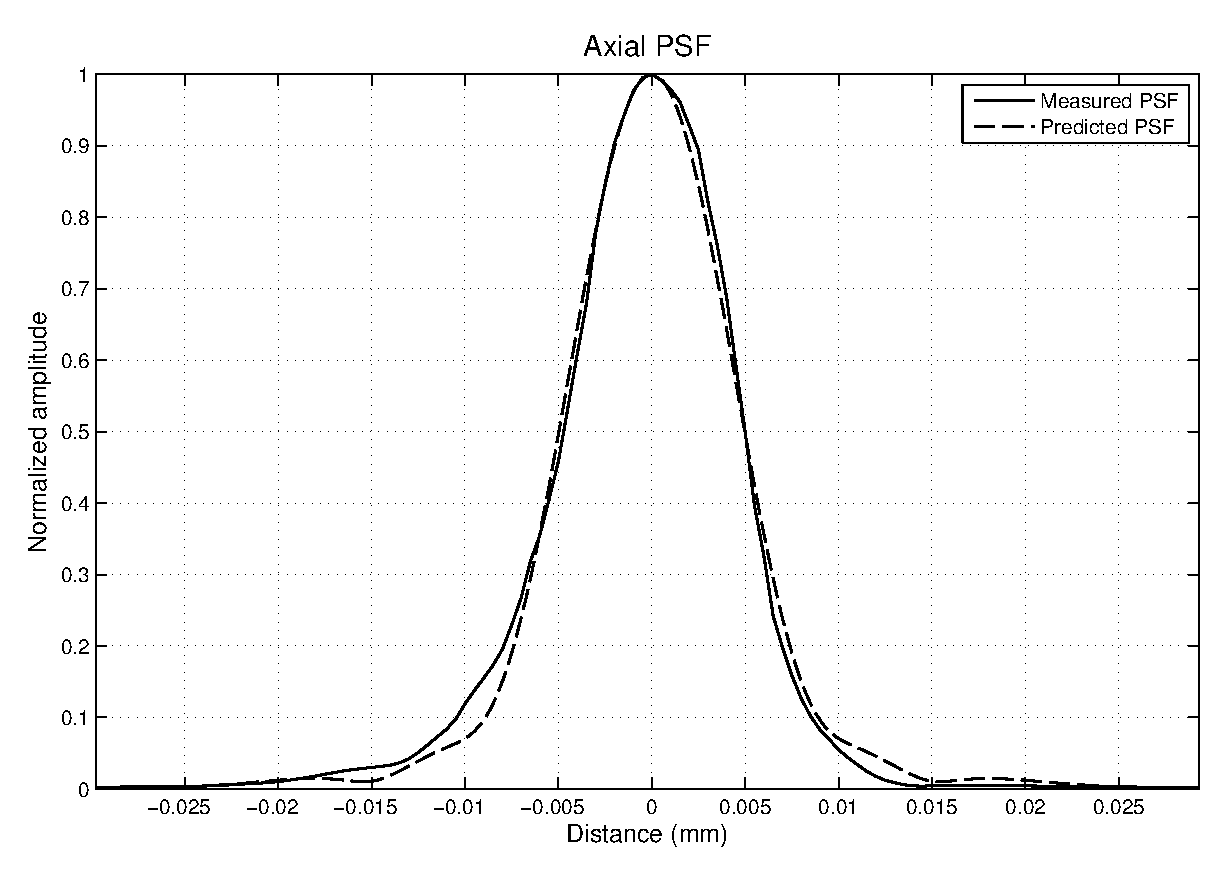
\includegraphics[width=0.8\textwidth]{Images/Results/psf-aom2.eps}
\caption[The measured axial point spread function.]{The measured axial point spread function of the FO-DOCM system. The measured PSF is shown as a solid line, and the predicted PSF as a dashed line.\label{fig:psf_comparison}}
\end{figure}

\subsection{Verification of transverse resolution}

Because the fiber DOCM system is not designed for en-face scanning, verifying the transverse resolution was significantly more difficult. To do so, two methods were used: an en-face scan of a standard USAF resolution test target, and a cross-sectional scan of the edge of a microscope coverslip.

Shown in Figure~\ref{fig:usaf}, the USAF resolution test target was imaged by holding the fiber DOCM system at a constant z-axis depth, and recording interferogram data while moving the y-axis continuously. Then, the x-axis was incremented by 1 micron, and the process repeats. Because the transverse stage was not choosen for suitability for this type of scanning, severe distortion is visible in the result due to the acceleration and deceleration of the stage during the y-axis scan. Vertical re-alignment of each column was performed to correct for poor repeatability in the stage, and a median filter was applied to reduce noise. While this method of scanning is clearly unsuitable for imaging applications, the visibility of all elements of group 6 within the USAF resolution test target do indicate a transverse resolution of approximately 8.8 microns.

\begin{figure}[h!]
\centering
\includegraphics[width=0.5\textwidth]{Images/Results/en-face-usaf.png}
\caption[Result of en-face scan of USAF target.]{Result of en-face scan of USAF target. Note the distortion caused by the variable speed and low repeatability on the transverse stepper motor stage. Despite the distortion, all of the elements of Group 6 are distinguishable, indicating a transverse resolution of approximately 8.8 microns.\label{fig:usaf}}
\end{figure}

To obtain a less distorted picture of the transverse resolution of the fiber DOCM system, a second experiment was performed. In this experiment, shown in Figure~\ref{fig:coverslip1}, the edge of a microscope coverslip, resting on a microscope slide, was imaged in the x-z plane. The transition between the coverslip and air is therefore the transverse step funtion of the system. Theoretically, this step function could be differentiated to obtain the transverse point spread function (PSF). However, differentiation increases noise, which renders this PSF unsuitable. Instead, the integral of a Gaussian function, an error function, can be fit to the step function, as shown in Figure~\ref{fig:coverslip2}. The best fit parameters correspond to a transverse FWHM of $9 \pm 0.7$ microns, which corroborates the USAF target image.

\begin{figure}[h!]
\centering
\includegraphics[height=230pt]{Images/Results/coverslip_ann.png}
\includegraphics[height=230pt]{Images/Results/coverslip_equal.png}
\caption[Result of scan of the edge of a a glass coverslip.]{Result of scan of the edge of a a glass coverslip, with major features labeled. On the right is the same image, with 1:1 scaling between the x and z axes.\label{fig:coverslip1}}
\end{figure}

\begin{figure}[h!]
\centering
\includegraphics[width=0.7\textwidth]{Images/Results/line_step.png}
\caption[Transverse step function measured along the glass coverslip.]{Transverse step function measured along the glass coverslip. This corresponds to a single horizontal line in Figure~\ref{fig:coverslip1}. The best fit error function (the integral of a Gaussian) corresponds to a FWHM resolution of $9 \pm 0.7$ microns, corroborating the USAF target experiment.\label{fig:coverslip2}}
\end{figure}

\subsection{Verification of motion resolution}

\begin{figure}[h!]
\centering
\includegraphics[width=0.75\textwidth]{Images/Results/noise_floor_r1_sm.png}
\caption[Noise floor of motion measurement with sample reflectivity of approximately $1$.]{Noise floor of motion measurement with sample reflectivity of approximately $1$. The noise floor above 2 KHz is approximately 2 pm/Hz$^{0.5}$. The peaks near 2 KHz, 20 KHz, 60 KHz, and 130 KHz are the result of electromagnetic interference between the ADC and the computer hosting it. \label{ref:noise_floor1}}
\end{figure}

To verify motion resolution, the sample path was focused onto a stationary mirror. The acquired photodiode signal was analyzed according to the process outlined in Section~\ref{sec:motion_analysis_2}. The spectral density noise floor of this signal is shown in Figure~\ref{fig:noise_floor1}. The strong impulsive frequencies present were believed to be caused by electromagnetic interference in the analog-to-dicigital converter, and not any inherent issues with the FO-DOCM system. % justify this?
Above approximately 2 KHz, the effective noise floor for motion resolution with a sample reflectivity of 1 is shown to be 2 pm/Hz$^{0.5}$.

To more accurately simulate the reflectivity of tissues, a $10^{-3}$ attenuator was inserted into the optical path, attenuating the sample signal by $10^{-6}$. 

\begin{figure}[h!]
\centering
\includegraphics[width=0.75\textwidth]{Images/missing.png}
\caption[Noise floor of motion measurement with sample reflectivity of approximately $10^{-6}$.]{Noise floor of motion measurement with sample reflectivity of approximately $10^{-6}$. The noise floor above 2 KHz is approximately XXX pm/Hz$^{0.5}$. The peaks near 2 KHz, 20 KHz, 60 KHz, and 130 KHz are the result of electromagnetic interference between the ADC and the computer hosting it. \label{ref:noise_floor2}}
\end{figure}

% These results are competitive with the Hong system.

\subsection{Resolution of motion differentiation}

The final system verification characteristic is referred to as ``motion diffferentiation resolution'' -- the ability of the system to resolve the difference in vibrational amplitude between closely spaced objects. For this experiment, a glass coverslip was held just above a piezo electric crystal, and the distance between the crystal and the coverslip was gradually reduced, as the displacement signal was analyzed.

\begin{figure}[h!]
\centering
\includegraphics[width=0.75\textwidth]{Images/missing.png}
\caption{Motion of vibrating and stationary interfaces measured with DOCM.}
\end{figure}

\section{Demonstrative images and motion measurements}

\begin{figure}[h!]
\centering
\includegraphics[width=1.0\textwidth]{Images/missing.png}
\caption{A comparison of a fixed cochlea scanned with the older Hong DOCM system (on the left), and the FO-DOCM system (on the right).}
\end{figure}

% Table indicating motion measurements from this fixed cochlea.

\section{Known issues and acknowledged shortcomings}


%\subsection{Motion of piezo-motor stage}

\section{Conclusion}